\section{Introduction}\label{sec:introduction}

Many industrial tasks on the edge of automation require a degree of adaptability that is difficult to achieve with conventional robotic automation techniques.
While standard control methods, such as PID controllers, are heavily employed to automate many tasks in the context of positioning, tasks that require significant adaptability or tight visual perception-control loops are often beyond the capabilities of such methods, and therefore are typically performed manually.
Standard control methods can struggle in presence of complex dynamical phenomena that are hard to model analytically, such as complex contacts.
Reinforcement learning (RL) offers a different solution, relying on trial and error learning instead of accurate modeling to construct an effective controller.
RL with expressive function approximation, i.e. deep RL, has further shown to automatically handle high dimensional inputs such as images \cite{mnih2013atari}.

However, deep RL has thus far not seen wide adoption in the automation community due to several practical obstacles. 
Sample efficiency is one obstacle: tasks must be completed without excessive interaction time or wear and tear on the robot. Progress in recent years on developing better RL algorithms has led to significantly better sample efficiency, even in dynamically complicated tasks \cite{haarnoja2018sac, hessel2018rainbow},
but remains a challenge for deploying RL in real-world robotics contexts.
Another major, often underappreciated, obstacle is goal specification: while prior work in RL assumes a reward signal to optimize,
it is often carefully shaped to allow the system to learn \cite{ng1999rewardshaping, popov17stacking, daniel2014activereward}. 
Obtaining such dense reward signals can be a significant challenge, as one must additionally build a perception system that allows computing dense rewards on state representations. Shaping a reward function so that an agent can learn from it is also a manual process that requires considerable manual effort. An ideal RL system would learn from rewards that are natural and easy to specify.
How can we enable robots to autonomously perform complex tasks without significant engineering effort to design perception and reward systems?

\begin{figure}[t]
    \centering
    \begin{subfigure}{0.14\linewidth}
        \center
        USB \vspace{1.1cm}
        
        D-Sub \vspace{1.1cm}
        
        Model-E
    \end{subfigure}
    \begin{subfigure}{0.14\linewidth}
        \center
        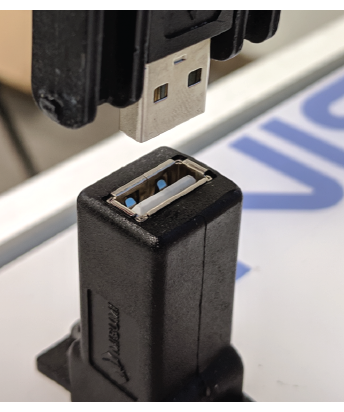
\includegraphics[height=1.17cm]{insertion/newfigs/usb.png} \vspace{0.2cm}
        
        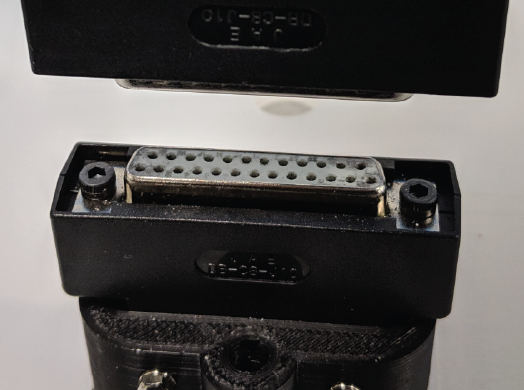
\includegraphics[height=1.17cm]{insertion/newfigs/dsub.png} \vspace{0.2cm}
        
        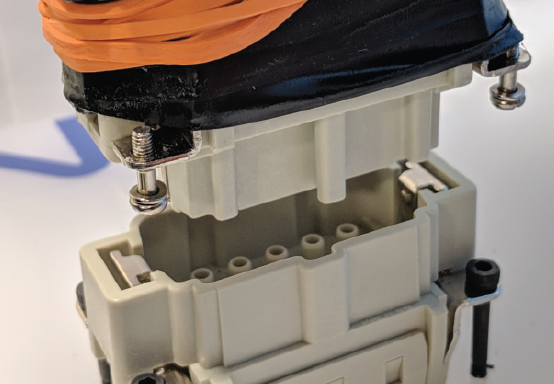
\includegraphics[height=1.17cm]{insertion/newfigs/modele.png} \vspace{0.05cm}
    \end{subfigure}
    \begin{subfigure}{0.69\linewidth}
        \begin{subfigure}[b]{0.69\linewidth}
            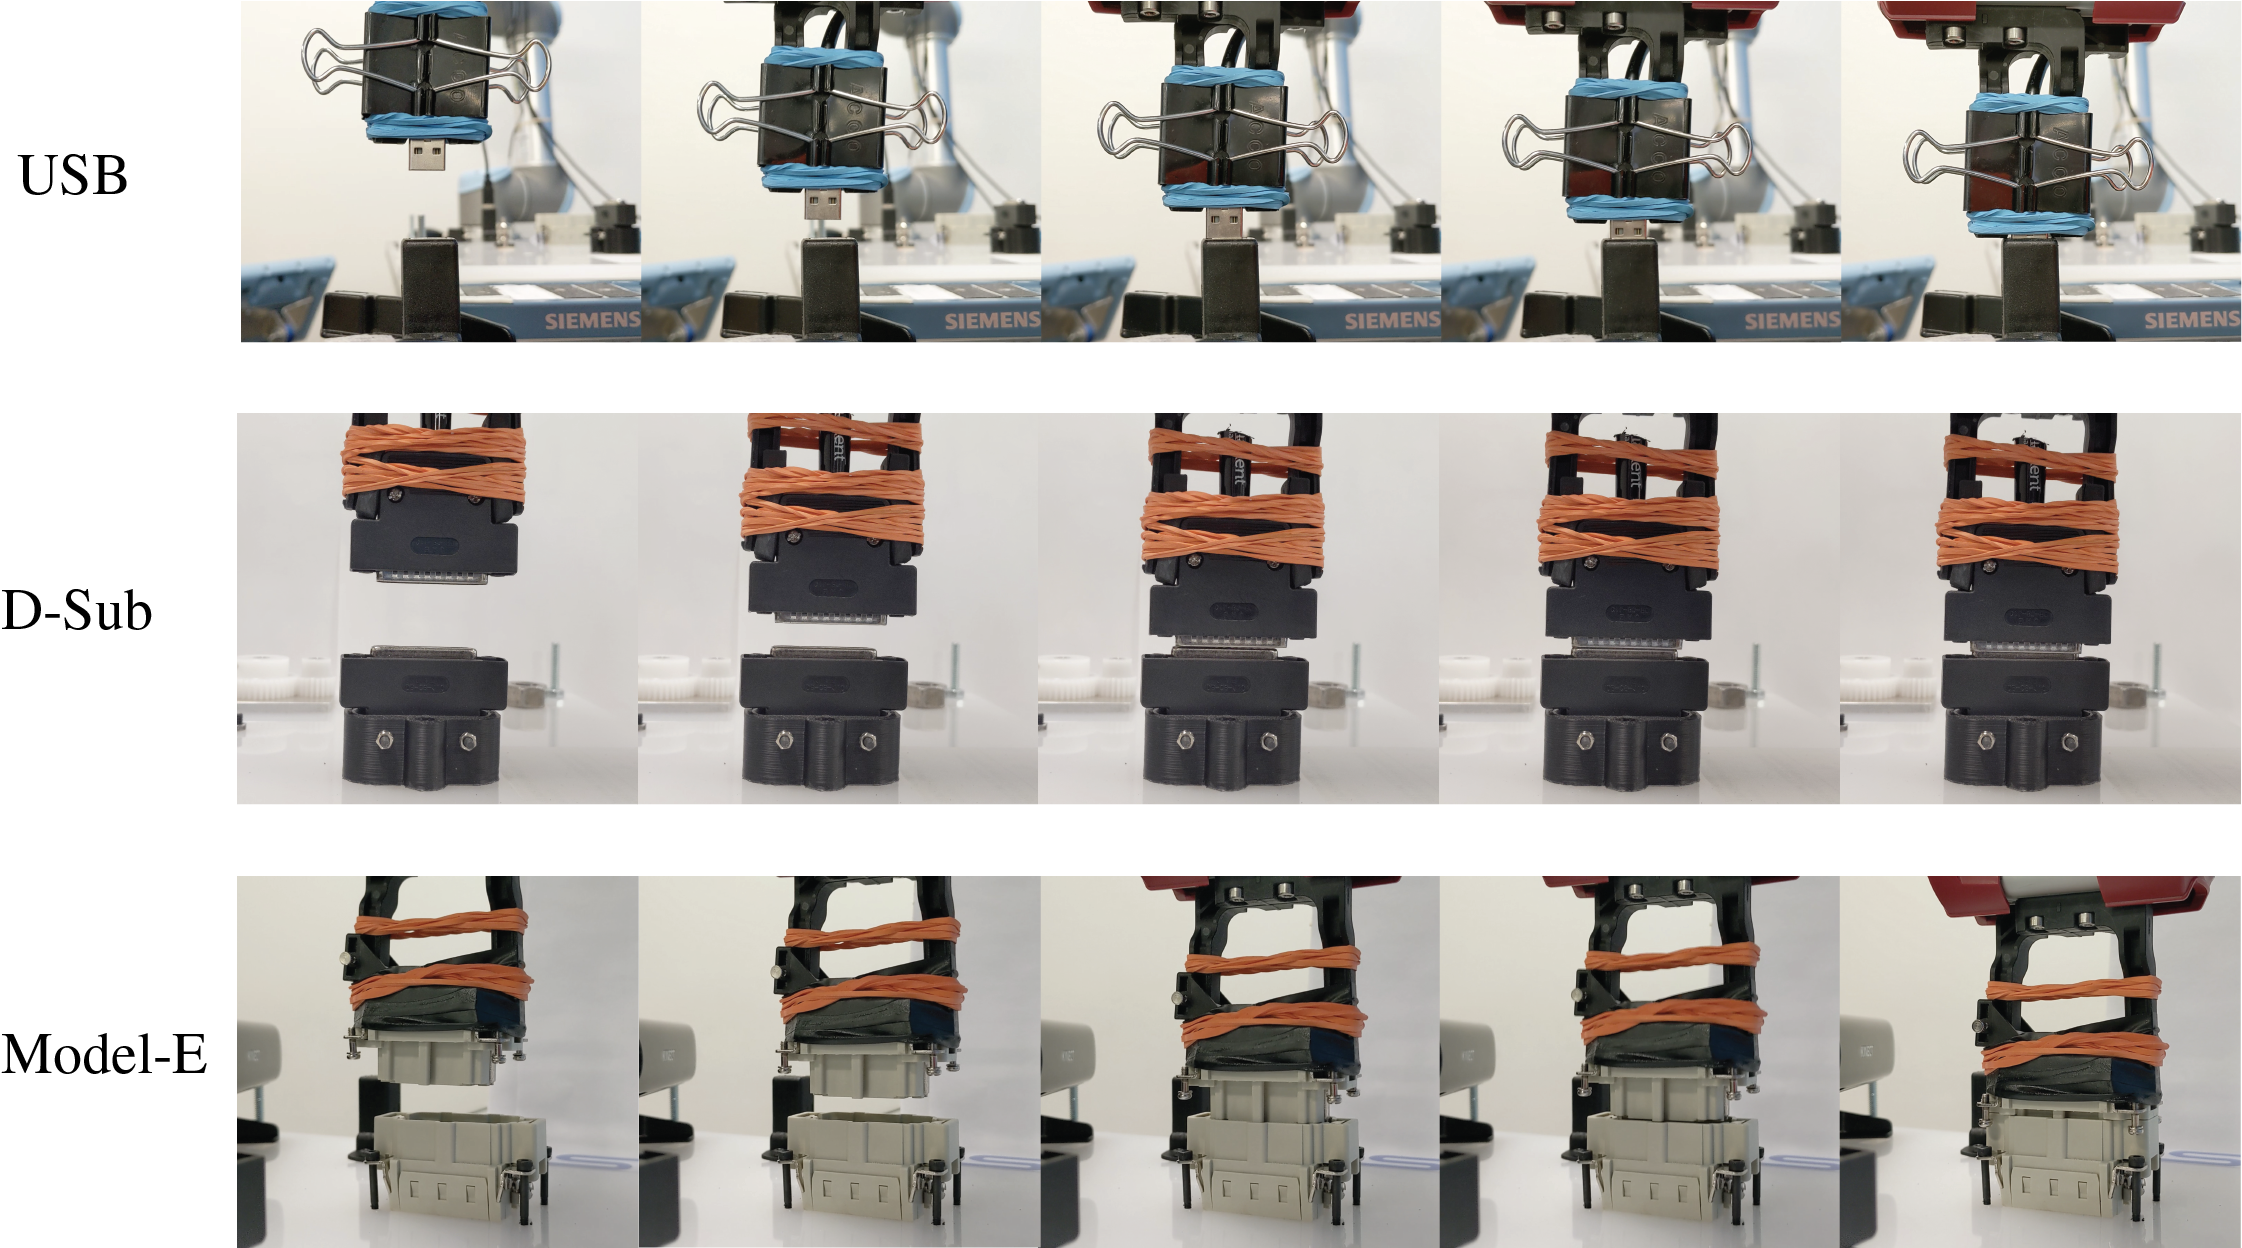
\includegraphics[trim={1.7cm 0 0 0},clip,width=0.99\linewidth]{insertion/newfigs/fig_usb.png} 
            \centering
        \end{subfigure}\hspace{2pt}
        \begin{subfigure}[b]{0.29\linewidth}
            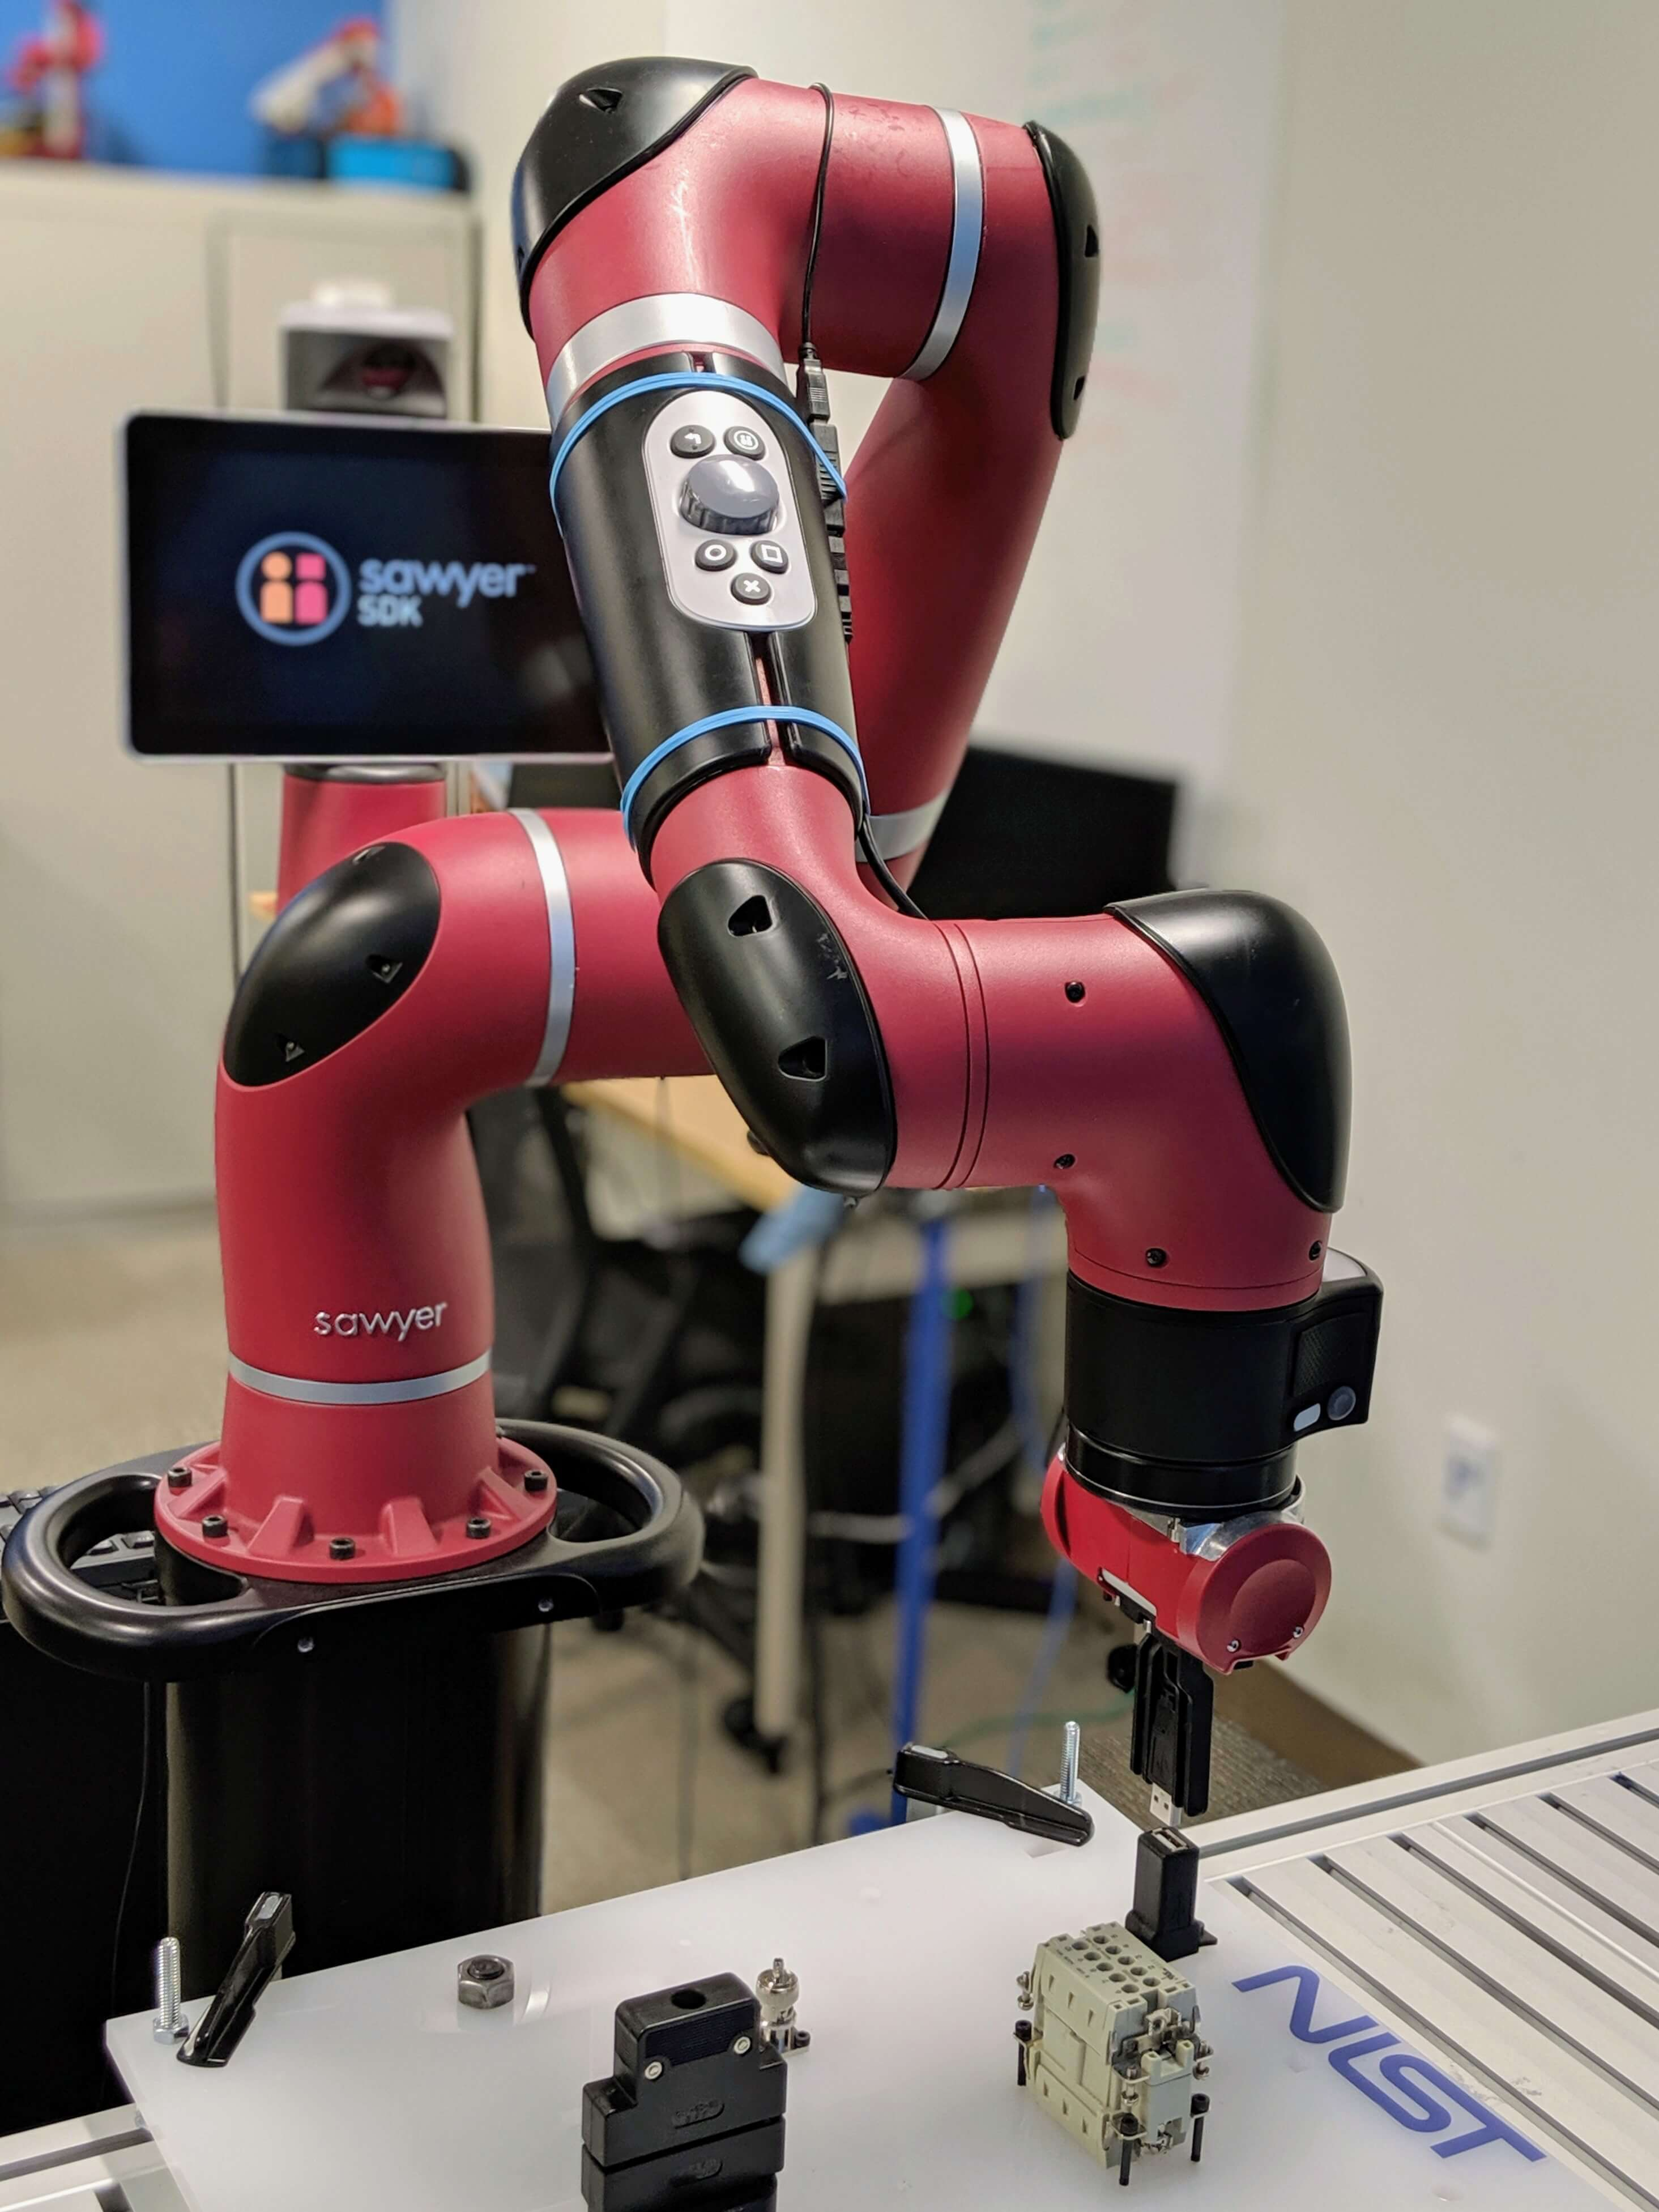
\includegraphics[trim={0 0 9cm 0},clip,width=0.99\linewidth]{insertion/figs/robot_view2.jpg}
            \centering
        \end{subfigure}\hfill
    \end{subfigure}

\caption{We train policies directly in the real world to solve connector insertion tasks from raw pixel input and without access to ground-truth state information for reward functions. Left: top-down views of the connectors. Middle: a rollout from a learned policy that successfully completes the insertion task for each connector is shown. Right: a full view of the robot setup. Videos of the results are available at \href{https://industrial-insertion-rl.github.io/}{industrial-insertion-rl.github.io} }
    \label{fig:usb_photo_demo2}
\end{figure}

We first consider an end-to-end approach that learns a policy from images, where the images serve as both the state representation and the goal specification. Using goal images is not fully general, but can successfully represent tasks when the task is to reach a final desired state \cite{nair2018rig}.
Specifying goals via goal images is convenient, and makes it possible to specify goals with minimal manual effort. Using images as the state representation also allows a robot to learn behaviors that utilize direct visual feedback, which provides some robustness to sensor and actuator noise.

Secondly, we consider learning from simple and sparse reward signals. Sparse rewards can often be obtained conveniently, for instance from human-provided labels or simple instrumentation. In many electronic assembly tasks, which we consider here, we can directly detect whether the electronics are functional, and use that signal as a reward. Learning from sparse rewards poses a challenge, as exploration with sparse reward signals is difficult, but by using sufficient prior information about the task, one can overcome this challenge. To handle this challenge, we extend the residual RL approach~\cite{johannink18residualrl, silver18residualpolicylearning}, which learns a parametric policy on top of a fixed, hand-specified controller, to the setting of vision-based manipulation.

% \begin{figure}[t]
%     \centering
%         \begin{subfigure}[b]{0.70\linewidth}
%             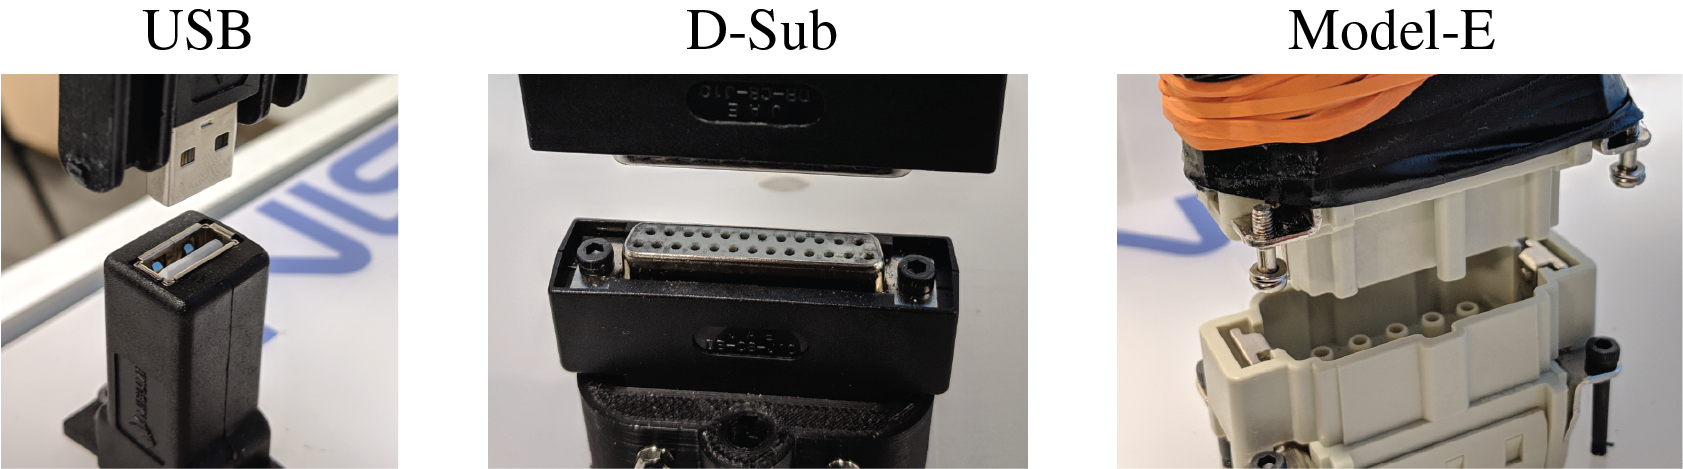
\includegraphics[width=0.99\linewidth]{insertion/newfigs/fig_ports.png} 
%             \centering
%         \end{subfigure}%\hfill
    
%     \caption{A close-up view of the three connector insertion tasks shows the contacts and tight tolerances the agent must navigate to solve these tasks. These tasks require sub-millimeter precision without visual feedback. }
%     \label{fig:usb_photo_demo}
% \end{figure}

In our experiments, we show that we can successfully complete real-world tight tolerance assembly tasks, such as inserting USB connectors, using RL from images with reward signals that are convenient for users to specify.
We can learn from only a sparse reward based on the electrical connection for a USB adapter plug, and we demonstrate learning insertion skills with rewards based only on goal images.
These reward signals require no extra engineering and are easy to specify for many tasks. 
Beyond showing the feasibility of RL for solving these tasks, we evaluate multiple RL algorithms across three tasks and study their robustness to imprecise positioning and noise.
